\documentclass[12pt]{scrartcl}
\usepackage[sexy]{james}
\usepackage[noend]{algpseudocode}
\setlength{\marginparwidth}{2cm}
\usepackage{answers}
\usepackage{array}
\usepackage{tikz}
\newenvironment{allintypewriter}{\ttfamily}{\par}
\usepackage{listings}
\usepackage{xcolor}
\usetikzlibrary{arrows.meta}
\usepackage{graphicx}
\usepackage{color}
\usepackage{mathtools}
\newcommand{\U}{\mathcal{U}}
\newcommand{\E}{\mathbb{E}}
\usetikzlibrary{arrows}
\Newassociation{hint}{hintitem}{all-hints}
\renewcommand{\solutionextension}{out}
\renewenvironment{hintitem}[1]{\item[\bfseries #1.]}{}
\renewcommand{\O}{\mathcal{O}}
\declaretheorem[style=thmbluebox,name={Chinese Remainder Theorem}]{CRT}
\renewcommand{\theCRT}{\Alph{CRT}}
\setlength\parindent{0pt}
\usepackage{sansmath}
\usepackage{pgfplots}

\usetikzlibrary{automata}
\usetikzlibrary{positioning}  %                 ...positioning nodes
\usetikzlibrary{arrows}       %                 ...customizing arrows
\newcommand{\eqdef}{=\vcentcolon}
\newcommand{\tr}{{\rm tr\ }}
\newcommand{\im}{{\rm Im\ }}
\newcommand{\spann}{{\rm span\ }}
\newcommand{\Col}{{\rm Col\ }}
\newcommand{\Row}{{\rm Row\ }}
\newcommand{\dint}{\displaystyle\int}
\newcommand{\dt}{\ {\rm d }t}
\newcommand{\PP}{\mathbb{P}}
\newcommand{\V}{\text{Var}}
\newcommand{\Cov}{\text{Cov}}
\newcommand{\horizontal}{\par\noindent\rule{\textwidth}{0.4pt}}
\usepackage[top=3cm,left=3cm,right=3cm,bottom=3cm]{geometry}
\newcommand{\mref}[3][red]{\hypersetup{linkcolor=#1}\cref{#2}{#3}\hypersetup{linkcolor=blue}}%<<<changed

\tikzset{node distance=4.5cm, % Minimum distance between two nodes. Change if necessary.
         every state/.style={ % Sets the properties for each state
           semithick,
           fill=cyan!40},
         initial text={},     % No label on start arrow
         double distance=4pt, % Adjust appearance of accept states
         every edge/.style={  % Sets the properties for each transition
         draw,
           ->,>=stealth',     % Makes edges directed with bold arrowheads
           auto,
           semithick}}


% Start of document.
\newcommand{\sep}{\hspace*{.5em}}

\pgfplotsset{compat=1.18}
\begin{document}
\title{BUFN402 Homework 1}
\author{James Zhang\thanks{Email: \mailto{jzhang72@terpmail.umd.edu}}}
\date{\today}

\definecolor{dkgreen}{rgb}{0,0.6,0}
\definecolor{gray}{rgb}{0.5,0.5,0.5}
\definecolor{mauve}{rgb}{0.58,0,0.82}

\lstset{frame=tb,
  language=Java,
  aboveskip=3mm,
  belowskip=3mm,
  showstringspaces=false,
  columns=flexible,
  basicstyle={\small\ttfamily},
  numbers=left,
  numberstyle=\tiny\color{gray},
  keywordstyle=\color{blue},
  commentstyle=\color{dkgreen},
  stringstyle=\color{mauve},
  breaklines=true,
  breakatwhitespace=true,
  tabsize=3
}

\maketitle

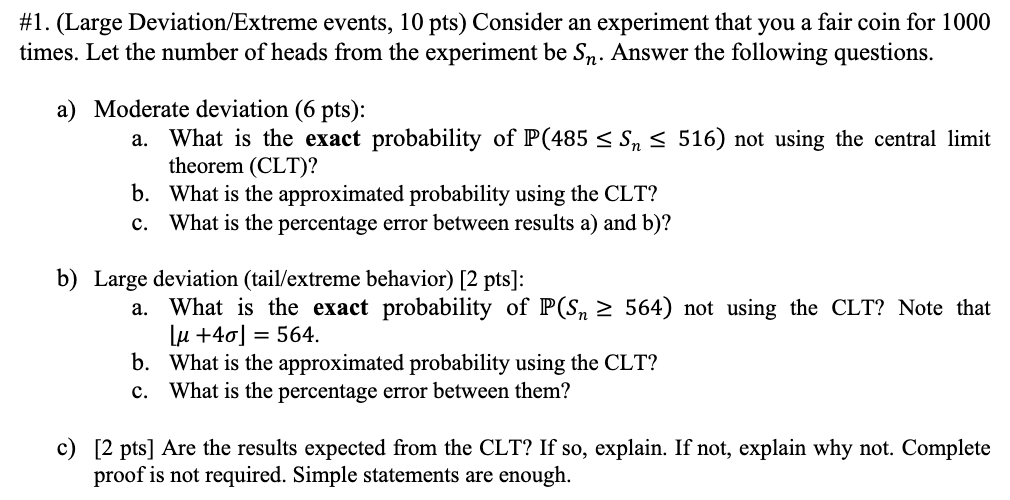
\includegraphics[width=15cm]{1.png}

\begin{proof}[Solution]
  
\hfill

\begin{enumerate}[a.]
  \item \begin{enumerate}[a.]

    \item Note that we can model repeated coin flips using a binomial random variable. Let 
    us denote this $X \sim \text{Binomial}(n=1000, p=0.5)$. The pmf of $X$ is 
    \[p(x) = \binom{n}{x}p^x(1-p)^{n-x}\]
    \[p(x) = \binom{1000}{x}(\frac{1}{2})^{1000}\]
    \[\PP(485 \leq S_n \leq 516) = \sum_{i=485}^{516} \binom{1000}{i}(\frac{1}{2})^{1000}\]
    \[\PP(485 \leq S_n \leq 516) \approx 0.8516 - 0.1795 = 0.6721\]

    \item Note that $\E(X) = np = 500$ and $\V(X) = np(1-p) = 250 \implies \sigma(X) = \sqrt{250}$. Using CLT
    
    \[\PP(485 \leq S_n \leq 516) = \PP(\frac{485 - 500}{\sqrt{250}} \leq \frac{S_n - 500}{\sqrt{250}} \leq \frac{516 - 500}{\sqrt{250}})\]
    \[= \phi(\frac{516 - 500}{\sqrt{250}}) - \phi(\frac{485 - 500}{\sqrt{250}}) = \phi(1.0119) - \phi(-0.9487)\]
    \[\approx 0.8442 - 0.1714 = 0.6728\]

    \item The percentage error is approximately 
    \[|\frac{0.6721 - 0.6728}{0.6721}| \approx 0.1402\% \text{ error}\]

  \end{enumerate}

  \item \begin{enumerate}[a.]
    \item The probability should be extremely low 
    given the fact that it is 4 standard deviations away. The exact probability of $\PP(S_n \geq 564)$ is 
    \[\PP(S_n \geq 564) = 1 - \PP(S_n < 564) = 1 - 0.99997 = 0.00003\]

    \item Using CLT, 
    \[1 - \PP(S_n < 564) = 1 - \PP(\frac{S_n - 500}{\sqrt{250}} < \frac{564 - 500}{\sqrt{250}}) = \phi(\frac{564 - 500}{\sqrt{250}})\]
    \[ = 1 - \phi(4.0477) = 1 - 0.99997 = 0.00003\]
    \item There is 0\% percentage error between the two calculations.
  \end{enumerate}

  \item The results are expected from the CLT because the given experiment satisfies the conditions of the CLT. 
  There are a 1000 samples, which is sufficient number of samples and the underlying Binomial distribution 
  has finite variance, which means the CLT can be applied. Thus, this Binomial distribution over the course of experiment 
  converges in distribution to a normal distribution.
\end{enumerate}

\end{proof}

\newpage

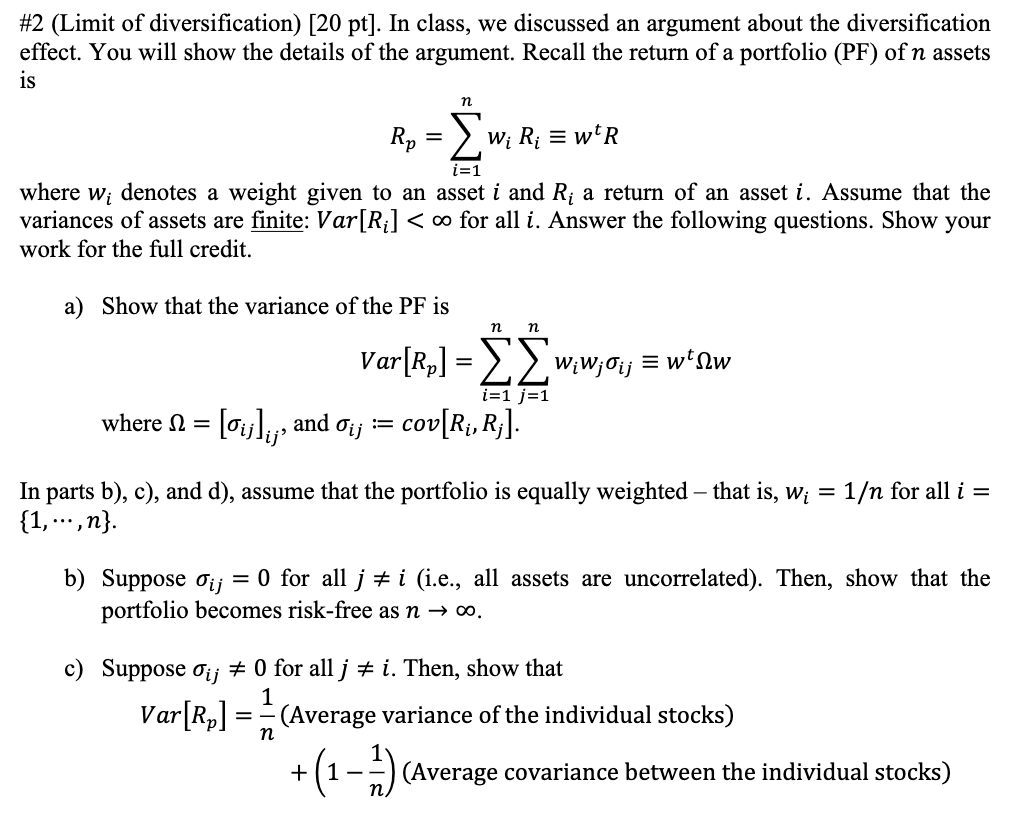
\includegraphics[width=15cm]{2.png}

\begin{proof}[Solution]

\hfill

\begin{enumerate}[a.]

\item To calculate the total variance of the portfolio $R_p$, 
\[\V(R_p) = \V(\sum_{i=1}^n w_i R_i)\]
Recall that variance does not follow linearity, and instead follows the property that 
\[\V(aX + bY) = a^2\V(X) + b^2\V(Y) + 2ab\Cov(X, Y)\]
For the case of $n$ assets, we write 
\[\V(\sum_{i=1}^n w_i R_i) = \sum_{i=1}^n w_i^2 \V(R_i) + 2\sum_{1 \leq i < j \leq n} w_i w_j\Cov(R_i, R_j)\]
Recall that $\V(R_i) = \Cov(R_i, R_i)$ and so we can rewrite it as
\[\V(R_p) = \sum_{i=1}^n \sum_{j=1}^n w_i w_j \Cov(R_i, R_j) = \sum_{i=1}^n \sum_{j=1}^n w_i w_j \sigma_{ij}\]
which is the first defined form. Note that this equivalent to the quadratic form, by definition of quadratic form,
and I will show this by considering the vector of weights and the covariance matrix.
\[\V(R_p) = w^T \Omega w = \begin{bmatrix}
  w_1 & \cdots & w_n
\end{bmatrix} \begin{bmatrix}
  \sigma_{11} & \cdots & \sigma_{1n}\\
  \vdots & \ddots & \vdots \\
  \sigma_{n1} & \cdots & \sigma_{nn}
\end{bmatrix} \begin{bmatrix}
  w_1 \\ \vdots \\ w_n
\end{bmatrix}\]
\[ = \begin{bmatrix}
  w_1 & \cdots & w_n
\end{bmatrix} \begin{bmatrix}
  w_1\sigma_{11} + \cdots + w_n\sigma_{1n}\\
  \vdots \\ 
  w_1\sigma_{n1} + \cdots w_n\sigma_{nn}
\end{bmatrix} = \begin{bmatrix}
  w_1 & \cdots & w_n
\end{bmatrix}
  \begin{bmatrix}
  \sum_{i=1}^n w_i \sigma_{1i}\\
  \vdots \\
  \sum_{i=1}^n w_i \sigma_{ni}
\end{bmatrix}\]
\[= w_1\sum_{i=1}^n w_i\sigma_{1i} + \cdots + w_n\sum_{i=1}^n w_i\sigma_{ni} = \sum_{i=1}^n \sum_{j=1}^n w_i w_j \sigma_{ij}\]
as desired.

\item Assuming equal weightings in all assets and covariances between all assets are exactly 0, 
then 
\[\V(R_p) = \V(\sum_{i=1}^n \frac{1}{n}R_i) = \frac{1}{n^2}\V(\sum_{i=1}^n R_i)\]
by a property of covariance. Now, taking the limit as $n\to\infty$, 
\[\lim_{n\to\infty}\frac{1}{n^2}\sum_{i=1}^n \V(R_i) = 0\]
which means the portfolio essentially becomes risk-free, as desired.

\item Now, assuming equal weightings in all assets but nonzero covariances, 
\[\V(R_p) = \sum_{i=1}^n \frac{1}{n^2} \V(R_i) + 2\sum_{1 \leq i < j \leq n} \frac{1}{n^2}\sigma_{ij}\]
\[\V(R_p) = \left(\frac{1}{n}\frac{1}{n}\sum_{i=1}^n \V(R_i)\right) + \left(2\sum_{i=1}^n \sum_{1 \leq i < j \leq n}^n \frac{1}{n^2}\sigma_{ij}\right)\]
\[\V(R_p) = \frac{1}{n}(\text{Average Variance}) + \frac{2}{n^2} * \binom{n}{2} * \frac{\sum_{i=1}^n \sum_{1 \leq i < j \leq n}^n \sigma_{ij}}{\binom{n}{2}}\]
where the N choose 2 follows from the fact that there are $\binom{N}{2}$ combinations of covariances 
between 2 assets. Note that therefore, the last term is simply the average covariance. 
Thus, 
\[\V(R_p) = \frac{1}{n}(\text{Average Variance}) + \frac{2}{n^2} * \frac{n(n-1)}{2}(\text{Average Covariance})\]
\[V(R_p) = \frac{1}{n}(\text{Average Variance}) + (1 - \frac{1}{n})(\text{Average Covariance})\]
as desired.
\end{enumerate}
  
\end{proof}

\newpage

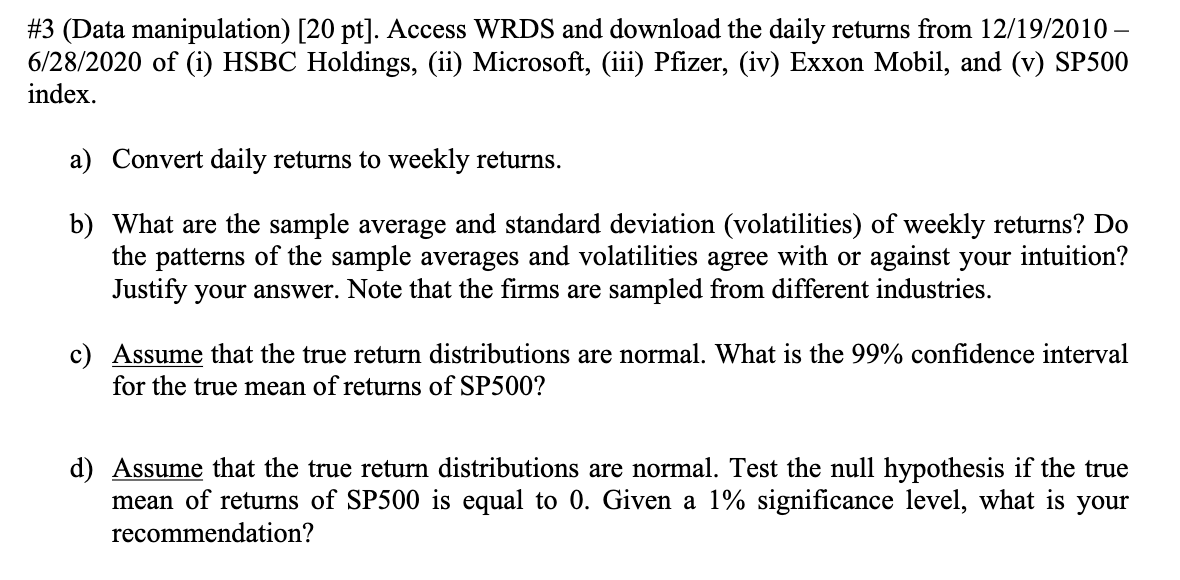
\includegraphics[width=15cm]{3.png}

\begin{proof}[Solution]

\hfill

Solution is written in the attached notebook.

\end{proof}

\newpage

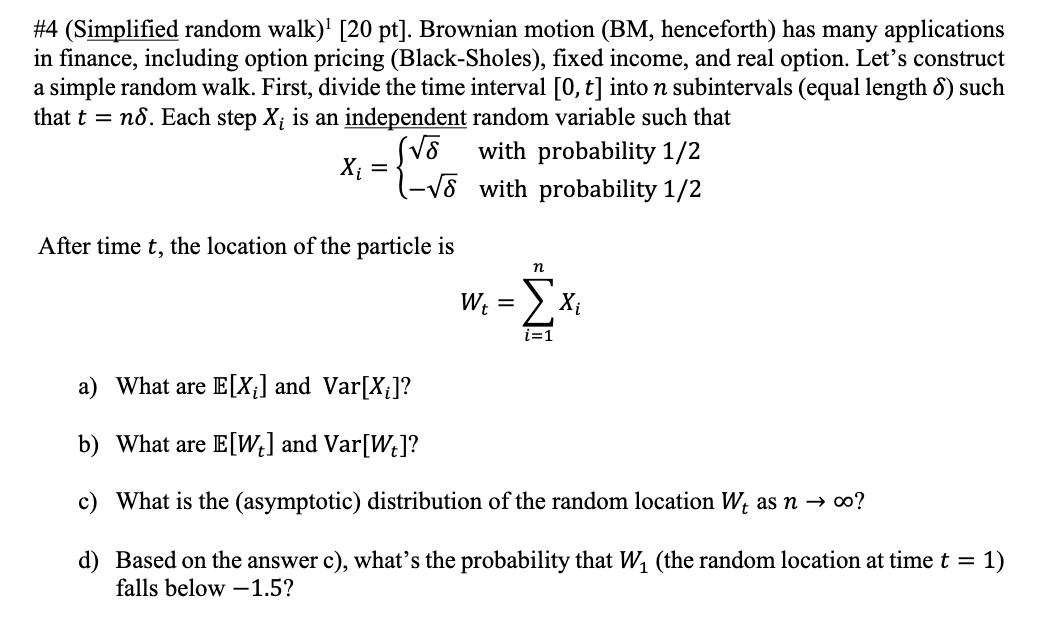
\includegraphics[width=15cm]{41.png}

\begin{proof}[Solution]
  
\hfill

\begin{enumerate}[a.]
\item $\E(X_i) = \frac{1}{2}\sqrt{\delta} + \frac{1}{2}(-\sqrt{\delta}) = 0$

$\V(X_i) = \E(X^2) - \E(X)^2 = \E(X^2) - 0 = \frac{1}{2}\delta + \frac{1}{2}\delta = \delta$

\item $\E(W_t) = \E(\sum_{i=1}^n X_i) = \sum_{i=1}^n \E(X_i) = 0$

$\V(W_t) = \V(\sum_{i=1}^n X_i) = \sum_{i=1}^n \V(X_i)$, since note that each $X_i$ is not scaled by a 
scalar and each $X_i$ is also an independent random variable, meaning $\Cov(X_i, X_j) = 0 \ \forall \ i \neq j$. 
Therefore, 
\[Var(W_t) = n\delta\]

\item Note that $t$ is fixed such that $t = n\delta$. Therefore, as $n\to\infty \implies \delta \to 0$. Thus, 
by the Central Limit Theorem, considering that we are interested in the asymptotic distribution 
of the sum and not a standardized sum, the asymptotic distribution $W_t = \sum_{i=1}^n X_i$ is 
\[W_t \sim N(0, n\delta) = N(0, t)\] 

\item At time $t=1, W_t \sim N(0, 1)$, so we just seek 
\[\phi(-1.5) \approx 0.0668\]

\item Shown in attached notebook.
\item Shown in attached notebook.
\item Shown in attached notebook.
\item Shown in attached notebook.
\end{enumerate}

\end{proof}

\newpage

All parts of problem 5 are answered in the attached notebook.
\end{document}

